\documentclass[12pt,a4paper]{report}
\setlength{\oddsidemargin}{0.25in}
\setlength{\evensidemargin}{0.15in}
\setlength{\topmargin}{0.1in}
\setlength{\textwidth}{6.0in}
\setlength{\textheight}{8.5in}
\usepackage{amsmath,amssymb}
\usepackage{graphics}
\usepackage{lscape,graphicx}
\usepackage{amsfonts}
\usepackage{longtable}
\usepackage{epsfig}
\usepackage{float}
\usepackage{rotating}
\usepackage{fancyhdr}
\setlength{\headheight}{14.5pt}
\usepackage[titletoc]{appendix}
\usepackage[english]{babel}
\addto{\captionsenglish}{\renewcommand{\bibname}{References}}

\usepackage{titlesec}
\usepackage{comment}

\usepackage{hyperref}
\hypersetup{
    colorlinks=true,
    linkcolor=red,
    filecolor=magenta,      
    urlcolor=black,
    % pdftitle={Overleaf Example},
    % pdfpagemode=FullScreen,
    }

%for pythia code 
% \usepackage{minted}
% %\usepackage{listings}% http://ctan.org/pkg/listings
% \lstset{
%   basicstyle=\ttfamily,
%   mathescape
% }
\usepackage{color}

\definecolor{dkgreen}{rgb}{0,0.6,0}
\definecolor{gray}{rgb}{0.5,0.5,0.5}
\definecolor{mauve}{rgb}{0.58,0,0.82}
\definecolor{ballblue}{rgb}{0.13, 0.67, 0.8}
\definecolor{cinnamon}{rgb}{0.82, 0.41, 0.12}
\definecolor{darkmagenta}{rgb}{0.55, 0.0, 0.55}
\definecolor{ferrarired}{rgb}{1.0, 0.11, 0.0}
\definecolor{mediumorchid}{rgb}{0.73, 0.33, 0.83}
\definecolor{mediumspringgreen}{rgb}{0.0, 0.98, 0.6}
\definecolor{orange}{rgb}{1.0, 0.5, 0.0}
\definecolor{magenta}{rgb}{1.0, 0.0, 1.0}
\usepackage[colorinlistoftodos]{todonotes}
%\usepackage[colorlinks,allcolors=black,bookmarks=ture,hypertexnames=true]{hyperref} 


% \lstset{frame=tb,
%   language=C++,
%   aboveskip=1mm,
%   belowskip=1mm,
%   showstringspaces=false,
%   columns=flexible,
%   basicstyle={\small\ttfamily},
%   numbers=none,
%   numberstyle=\tiny\color{sepia},
%   keywordstyle=\color{blue},
%   commentstyle=\color{dkgreen},
%   stringstyle=\color{mediumorchid},
%   %stringstyle=\color{International orange},
%   breaklines=true,
%   breakatwhitespace=true,
%   tabsize=1
% }



\titlespacing*{\chapter}{0pt}{0pt}{0pt}
\titleformat{\chapter}[display]{\normalfont\huge\bfseries}{}{10pt}{\Huge}

%\titleformat{\chapter}[display]{\normalfont\huge\bfseries}{
%\chaptertitlename\ \thechapter}{20pt}{\Huge}


%%%%%%%%%%%%%%%%%%%%%%%%%%%%%%%%%%%%%%%%%%
%%%  macro for margin change
\newenvironment{changemargin}[2]{%
\begin{list}{}{%
%\setlength{\topsep}{0pt}%
\setlength{\leftmargin}{#1}%
\setlength{\rightmargin}{#2}%
%\setlength{\listparindent}{\parindent}%
%\setlength{\itemindent}{\parindent}%
%\setlength{\parsep}{\parskip}%
}%
\item[]}{\end{list}}
%%%%%%%%%%%%%%%%%%%%%%%%%%%%%%%%%%%%%%%%%%

\begin{document}
\begin{changemargin}{0cm}{0cm}
\thispagestyle{empty}
\baselineskip25pt
\begin{center}
{\Large {\bf Kinematic study  in FCCee CLD detector}}\\
\end{center}

\vfill
\baselineskip15pt
\begin{center}
{\em  Report submitted by} \\

%\vskip .10\baselineskip

\end{center}
\baselineskip25pt

\vfill
\begin{center} %{\bf {\em by}} \\
{\large{\bf Pradyot pritam sahoo}} \\
{\large{ Roll No: 1811106}} \\
\vspace{20pt}

\textit{supervised by }\\
{\large{\bf Dr. Prolay kumar mal}} \\

\end{center}

\vfill
\begin{center}
\begin{figure}[h!]
\centering
\includegraphics[scale=0.2]{logo1.jpg}
% Reference for the Logo: Student Forms | NISER https://www.niser.ac.in/forms/academic/LaTexTemplate_MScThesis.zip
\end{figure}
 {\bf {\em to the }} \\
{\bf {\large School of Physical Sciences}} \\
{\bf {\large National Institute of Science Education and Research}} \\
{\bf Bhubaneswar} \\
{\bf \today} 
\end{center}
\end{changemargin}



\pagenumbering{roman}
\baselineskip=20pt
%\include{dedicate}
%\include{declaration}
%\include{stat}
%\include{cert1}
%\begin{center}
{\bf ACKNOWLEDGEMENTS}
\end{center}
I would like to thank my  guide Dr. Prolay kumar mal, for his guidance throughout this project.

%\begin{center}
{\large {\bf  ABSTRACT }}
\end{center}  

Higgs-strahlung $e^{+} + e^{-}\longrightarrow Z+H$ is the most important mechanisms for the production of Higgs bosons in  $e^{+} + e^{-}$ collisions at $LEP$ and future $e^{+} + e^{-}$ linear colliders. We have calculated the different kinematic parameters such as transverse momentum, rapidity, pseudorapidity, etc. of the Higgs and Z boson using $PYTHIA$ event generator.
When the Z boson decays into $e^{+}e^{-}$ or $\mu^{+}\mu^{-}$,
we have calculated the angle between the daughter particles and also reconstruct the mass of the $Z$ boson from the daughter particle.
At last, we have calculated the angle between $Z$ and $Higgs$ in this which comes out to $\pi$ for conserving momentum.
%\clearpage

\fancyfoot{}      % Delete current footer settings
\pagestyle{fancyplain}
\renewcommand{\chaptermark}[1]{\markboth{\thechapter\ #1}{\thechapter\ #1}} % remember chapter title
\lhead[\fancyplain{}{}]{\fancyplain{}{}}
\rhead[\fancyplain{}{}]{\fancyplain{}{\em\leftmark }}
\renewcommand{\headrulewidth}{0.3pt}
\cfoot{\rm\thepage} % page number
\baselineskip=12pt

% \tableofcontents
% \clearpage
% \listoffigures
% \clearpage
% \listoftables 
% \clearpage
\pagenumbering{arabic}
\baselineskip=24pt

%\setlength {\marginparwidth }{2cm}

\chapter{\label{intro}Introduction}

\setcounter{equation}{0}
\setcounter{table}{0}
\setcounter{figure}{0}
\setcounter{chapter}{1}

\baselineskip 24pt
\hspace{10pt}
\\
Based on the work for a detector at CLIC, this report provides a conceptual description and illustration of the CLD detector. CLD is one of the detectors planned for a future 100-kilometer $e+e-$ linear circular collider (FCC-ee). The note also includes  a brief description of the simulation and
reconstruction tools used in the linear collider community, which have been adapted for
physics and performance studies of CLD. We have learned about detector description which is an 
essential component  to analyze data resulting from
particle collisions in high energy physics experiments.
 
In this project, We have selected the \emph{Higgs-Strahlung process}$(e^{+}+ e^{-}\longrightarrow Z+ 
H)$  by  $e^{+}e^{-}$ collision  at $240GeV$ center of mass energy. We have 
run a fast parametric detector simulation with Delphes in the EDM4Hep format
then applied  event selection on those samples with FCCAnalyses
and produced flat ntuples with observables of interest with FCCAnalyses.
Then we have analyzed the different kinematics of $Higgs$ and $Z$ boson and their daughter particles
with FCCAnalyses.

As we know $Z$ boson is the exchange particles mediating weak interaction, which can decay when it 
produces. We have only focused on two of the  detectable decay-modes, the decay into 
electron-positron$(e^{+}e^{-})$ or muon-antimuon$(\mu^{+}\mu^{-})$. 
We have studied different kinematic parameter such as energy$(E)$, transverse momentum$(p_T)$, 
momentum $(p)$, rapidity$(y)$, $\theta$ of daughter particle and  reconstructed its 
four momentum $(p^{\mu})$. In order to satisfies invariant mass law we have reconstructed the mass  of  $Z$ boson from their daughter particles.



% The toolkit will be built
% reusing already existing components from the ROOT geometry package and provides missing
% functional elements and interfaces to offer a complete and coherent detector description solution.
% A natural integration to Geant4, the detector simulation program used in high energy physics,
% is provided.


\chapter{\label{method}Description of CLD detectors$^{\cite{CLD}}$}

\setcounter{equation}{0}
\setcounter{table}{0}
\setcounter{figure}{0}

\baselineskip 20pt
\hspace{10pt}
\section{Dimension and layout}
In this following sections we have described the  possible future  CLD detector for 
FCC-ee \cite{CLD}. This detector  have  a silicon 
pixel vertex detector and a silicon tracker, followed by highly 
granular calorimeters (a silicon-tungsten ECAL and a 
scintillator-steel
HCAL). A superconducting solenoid provides a strong magnetic 
field, and a steel yoke interleaved with
resistive plate (RPC) muon chambers closes the magnetic field.
At this stage of the design of detector, it is assumed that the detector is identical for all the collision energies of FCC-ee, i.e. for operation at the $Z (91.2 GeV)$, $W (160 GeV)$, $H (240 GeV)$ and $top (365 GeV)$.
\begin{figure}
    \centering
    \includegraphics[width = 6.5cm, height = 5.5cm]{fcc_det/ph1.png}
    \caption{Isometric view of the CLD detector, with one quarter removed.}
    \label{fig:detector1}
\end{figure}

\begin{figure}
    \centering
    \includegraphics[width = 9cm, height = 9cm]{fcc_det/ph2.png}
    \caption{Vertical cross section showing the top right quadrant of CLD.}\label{fig:detector2}
\end{figure}

\begin{figure}
    \centering
    \includegraphics[width = 8cm, height = 9cm]{fcc_det/ph3.png}
    \caption{Transverse $(XY)$ cross section of CLD.}
    \label{fig:mymodel3}
\end{figure}

\section{Vertex detector}
The vertex detector in the CLD concept, a higher  version of the 
one in CLICdet, consists of a cylindrical
barrel detector closed off in the forward directions by discs. 
The layout is based on double layers, i.e.
two sensitive layers fixed on a common support structure (which 
includes cooling circuits). The barrel
consists of three double layers, the forward region is covered 
by three sets of double-discs on both sides
of the barrel. An overview of the vertex detector layout is 
given in Figure(\ref{fig:vertex}). The total area of the vertex
detector sensors is 0.53$m^2$.
\begin{figure}[ht]
    \centering
    \includegraphics[width = 1\linewidth]{fcc_det/ph14.png}
    \caption{Vertex detector layout in ZR plane. Red lines indicating sensors, black lines indicating support structure and vaccume pipe in orange color.}
    \label{fig:vertex}
\end{figure}


The vertex detector consists of 
$25\times25\mu$m$^2$ pixels 
having  a silicon sensor thickness of $50\mu$m. Using
pulse height information and charge sharing, a single point 
resolution of $3\mu$m is aimed for.
The overall length of the barrel vertex detector, built from staves, is 250 mm. The double layer
structure is shown in Figure(\ref{fig:vertex2}).
The vertex detector forward region consists of three discs on 
each side where  each disc is built as a double layer device. The 
discs are located a distance from the IP of 160, 230 and 300 
mm respectively. They are
constructed from 8 trapezoids, approximating a circle. For 
simplicity the trapezoids are not overlapping
in the simulation model. The inner radii of the forward discs 
respect the 150 mrad cone reserved for MDI elements. 
\begin{figure}
    \centering
    \includegraphics[width=6cm, height=6cm]{fcc_det/ph5.png}
    \caption{Vertex detector double layer structure in XY plane.}
    \label{fig:vertex2}
\end{figure}

\section{Silicon tracker}
Like  CLIC detector, the CLD concept have  an all-silicon tracker. 
The inner tracker consists of three barrel layers and seven forward discs. The outer tracker
has  an additional three barrel layers and four discs. The overall layout of the silicon tracker in CLD is shown in Figure(\ref{fig:tracking}) .
\begin{figure}[ht]
    \centering
    \includegraphics[width = 7cm, height = 7cm]{fcc_det/ph6.png}
    \caption{ Overall layout of the CLD tracking system: the vertex barrel detector is shown in yellow, the
    tracking layers in lighter red.  The surrounding ECAL is shown in green.}
    \label{fig:tracking}
\end{figure}
The tracking volume has a half-length of 2.2m and a maximum radius of 2.1m. This radius allows to
achieve a similar momentum resolution in the CLD tracking system with a 2T magnetic field as in the CLIC detector  tracker with a 4T field and a radius of 1.5 m. The main support tube has an inner and outer radius of 0.686m and 0.690m respectively, and a half-length of 2.3 m.
The
tracking system covers polar angles larger than 150 mrad.
The pixel vertex detector and the silicon tracker are treated as one unified tracking system in simulation and reconstruction.

\section{Electromagnetic calorimeter(ECAL)}
Further studies about  ILC and CLIC have revealed 
that high granularity particle flow calorimetry appears to be a 
promising option to reach the required jet energy resolution of 
3-4$\%$. Such a performance is necessary to allow the 
distinction e.g. of $W$ and $Z$ bosons on an event-by-event basis.
\begin{figure}[ht]
    \centering
    \includegraphics[width = 12cm, height = 3.5cm]{fcc_det/ph10.png}
    \caption{Schematic drawing of the ECAL segmentation as implemented in the simulation model}
    \label{fig:ecal}
\end{figure}
The segmentation of the ECAL has to be sufficient to resolve 
energy depositions from nearby particles in
high energy jets. Studies performed in the context of the ILC 
and CLIC suggest a calorimeter transverse
segmentation of $5 \times 5$mm$^2$.
The technology chosen as baseline option for the detectors at 
the linear colliders is a silicon-tungsten sandwich structure as shown in Figure(\ref{fig:ecal}).
This detector design is also implemented in the CLD simulation
model.


\section{Hadron calorimeter(HCAL)}
The  hadronic
calorimeter of CLD has a structure and granularity as the one 
in CLICdet. It consists of steel absorber
plates, each of them 19mm thick interleaved with scintillator 
tiles. The gap for the 
sensitive layers and their cassette is 7.5mm.
The polystyrene scintillator in the cassette is 3 mm thick with 
a tile size of $30 \times 30$ mm$^2$.
In the simulations,
the part of the HCAL endcap which surrounds the ECAL endcap  is 
treated as a separate
entity called the "HCAL ring". The detailed HCAL layer stack as implemented in the simulation 
model is shown in Figure(\ref{fig:hcal}).
\begin{figure}[ht]
    \centering
    \includegraphics[width = 12cm, height = 3.5cm]{fcc_det/ph11.png}
    \caption{ Schematic drawing of HCAL segmentation as implemented in the simulation model.
    }
    \label{fig:hcal}
\end{figure}


\section{Magnet system}
The solenoid magnetic field of the CLD detector  is 2T, 
which is limited by MDI constraints. 
In the simulation model, the magnetic field in CLD is 2T 
throughout the volume inside the superconducting coil. The 
field in the yoke barrel is 1T, pointing in the opposite 
direction with respect to the
inner field. The simulation model currently assumes no field in 
the yoke endcap nor outside the yoke.


\section{Muon system}
The iron  yoke is divided  into three rings in the barrel region and the two endcaps, as shown in
Figure(\ref{fig:muon}). The thickness of the yoke is reduced w.r.t. CLICdet, in correspondence to the lower solenoid
field . A muon identification system with 6 layers as in CLICdet is implemented. An additional 7th layer
is inserted in the barrel as close as possible to the coil. This layer may serve as tail catcher for hadron
showers. The muon system layout in CLD is shown in Figure(\ref{fig:yoke}).

\begin{figure}[ht]
    \centering
    \includegraphics[width=8cm, height=6cm]{fcc_det/ph12.png}
    \caption{Segmentation of the iron return yoke of CLD into endcaps and three barrel rings.}
    \label{fig:muon}
\end{figure}

\begin{figure}[ht]
    \centering
    \includegraphics[width = 7cm, height = 7cm]{fcc_det/ph13.png}
    \caption{ Schematic cross section of the muon system layout in the yoke of CLD.}
    \label{fig:yoke}
\end{figure}
%%\chapter{\label{results}Two-body decay kinematics}

%\setcounter{equation}{0}
%\setcounter{table}{0}
%\setcounter{figure}{0}
%\baselineskip 24pt
%\hspace{10pt}
%\\
\section{Kinematics}
\subsection{Four momentum}
\noindent
\begin{itemize}
    \item 
Relativistic kinematics problems are greatly simplified by using $4-$vectors,
for any $4-$momentum $p^{\mu}$ is given by,

\begin{equation}
    p^{\mu} = (E/c, \Vec{p})= (m\gamma c, m \gamma \Vec{u})
\end{equation}
\item
A four momentum equation automatically takes into account conservation of energy and momentum. For example, if a particle $X$ decays into two daughters,
we write the $4-$momentum equation will be
\begin{equation}
  P_{X}^\mu = p_{a}^\mu + p_{b}^\mu  
\end{equation}
\item Where the mass $M$ of the heavier particle is given by $p_{0}.p_{0}=M^2c^2$. By measuring the energy and momentum of the daughter particles, one can reconstruct the invariant mass of the two-particle system, which must be equal to $M$.
\end{itemize}
   
%%%%%%%%%%%%%%%%%%%%%%%%%%%%%%%%%%%%%%%%%%%%%%%%%%%%%%%%%%%%%%%%%%%%%%%%%%%%%%%%

\subsection{Particle decay in Center of mass frame}
Consider the decay of a particle$(X)$ with mass $M$ to two particles of mass $m_{a}$ and $m_{b}$ in the rest frame of the parent particle. 
Application of $4-$momentum conservation leaves us with just $2$ degrees of freedom. Two daughter particles must be emitted back
to back in the parent rest frame for conserving momentum.
\begin{figure}[h]
    \centering
    \includegraphics[width = 9cm, height = 5.5cm]{cm3.png}
    \caption{Particle decay in CM-frame}
    \label{fig:my_label}
\end{figure}
\hspace{10pt}
\\
\begin{itemize}
    \item 
In CM frame for $a$ and $b$ mother particle $X$ is at rest, so the $4-$momenta will be 
        \begin{equation}
            \textbf{p}_{X} = (M c,0,0,0), \textbf{p}_{a}= (E_{a}/c, \Vec{p}_{a}), \textbf{p}_{b}= (E_{b}/c, \Vec{p}_{b})
        \end{equation}
\item        
 Conservation of $4-$momentum requires the following 
\begin{equation}
    \textbf{p}_{X} = \textbf{p}_{a} + \textbf{p}_{b} \implies \Vec{p}_a = -\Vec{p}_b
\end{equation}    
        
\item    
 For energy conservation 
 \begin{equation}
     E_{a}+E_{b} = \sqrt{m_{a}^2c^4+p^2c^2}+ \sqrt{m_{b}^2c^4+p^2c^2} =M c^2
 \end{equation}

\end{itemize}

By solving the above relation we got the expression 
        \begin{equation}
            p = c\frac{\sqrt{[M^2-(m_{a}-m_{b}^2)][M^2-(m_a +m_b)^2]}}{2M}
        \end{equation}

Which results  
    \begin{equation}
         M \geq m_{a} + m_{b}
    \end{equation}

So, if the particle has greater mass than sum of masses of two daughter particles
particle is unstable and decays.  Momenta of daughter particles and energies fixed by $3$ masses
from energy conservation $E_{b}=\sqrt{E_{a}^2-m_{a}^2c^4+m_{b}^2c^4}$ solve to get that 
        \begin{equation}
            E_{a} = \frac{(M^2+m_{a}^2-m_{b}^2)c^{2}}{2M}
        \end{equation}
    similarly
        \begin{equation}
            E_{b} = \frac{(M^2+m_{b}^2-m_{a}^2)c^{2}}{2M}
        \end{equation}
There is no preferred direction in which the daughter particles travel. So decay is said to be isotropic in which daughter particles traveling back-to-back in $X$ rest frame.

%%%%%%%%%%%%%%%%%%%%%%%%%%%%%%%%%%%%%%%%%%%%%%%%%%%%%%%%%%%%%%%%%%%%%%%%%%%%%%%%%%%

\subsection{Particle decay in Lab frame}
Previously, we have determined energy and momentum  for two-body decay in the parent particle CM frame. However, we need to find their values in the frame where the parent particle is moving, e.g. the detector frame(Lab frame).  
\begin{figure}[h]
    \centering
    \includegraphics[width=11cm, height=5cm]{lab3.png}
    \caption{Particle decay in Lab-frame}
    \label{fig:my_label}
\end{figure}
\\
\noindent
\begin{itemize}
    \item 
By taking  $\hat{z}$-axis along direction of flight of mother particle, the $4-$momenta for  $a$, $b$ and  mother particle $X$ is at lab frame will be 
        \begin{equation}
            \textbf{p}_{X} = (E/c,0,0,p), \textbf{p}_{a}= (E_{a}/c, \Vec{p}_{a\perp}, p_{a z}), \textbf{p}_{b}= (E_{b}/c, \Vec{p}_{b\perp}, p_{b z})
        \end{equation}
\item        
By momentum conservation (transverse momentum vectors)
        \begin{equation}
            \Vec{p}_\perp \equiv \Vec{p}_{a\perp} =  -\Vec{p}_{b\perp} 
        \end{equation}
\item
Energies and $\hat{z}$ components of particle momenta
related to those in the CM-frame by a Lorentz boost
with a boost velocity equal to the speed of the mother particle along $\hat{z}$ direction is given by         
    \begin{equation}
    \begin{split}
                E_{a} =& \gamma (E^{*}_a/c + \beta p^{*}_{a z})\\
                p_{a z} =& \gamma (p^{*}_{a z}+\beta E_{a}^{*}/c)\\
                \Vec{p}_{a\perp} =& \Vec{p}_{a\perp}^{*}\\
    \end{split}
    \end{equation}
similarly for $b$ particle, 
    \begin{equation}
    \begin{split}
                E_{b} =& \gamma (E^{*}_b/c + \beta p^{*}_{b z})\\
                p_{b z} =& \gamma (p^{*}_{b z}+\beta E_{b}^{*}/c)\\
                \Vec{p}_{b\perp} =& \Vec{p}_{b\perp}^{*}\\
                \beta = p c/ E  \  \ &and  \ \ \gamma = E/ (M c^{2}) 
    \end{split}
    \end{equation}
\end{itemize}

\noindent    
This completely solves problem
from which we can find angles $(\theta)$ which daughter particles
make with $z$-axis and with each other as functions of $p_{X}$.

\begin{figure}[h]
    \centering
    \includegraphics[width=12cm, height=4cm]{1.png}
    \caption{Comparison between CM frame$(S)$ and Lab frame$(S^\prime)$}
    \label{fig:my_label}
\end{figure}
\begin{itemize}
    \item 
In $S$ frame(Rest frame) four momentum is given by  
    \begin{equation}
        p^{\mu} = (E/c, p \cos{\theta}, p\sin{\theta}, 0)
    \end{equation}
\item
In $S^{\prime}$(boosted frame) it follows as 
    \begin{equation}
        p^{\prime\mu} = (E^\prime/c, p^\prime \cos{\theta^\prime}, p^\prime\sin{\theta^\prime}, 0)
    \end{equation}
\end{itemize}
\noindent

Applying $S \longrightarrow S^{\prime}$ Lorentz transformation
\begin{equation}
    \begin{split}
        p^{\prime}\cos{\theta^{\prime}} = & \gamma^{*}(p\cos{\theta}-\beta^{*}E/c)\\
        p^{\prime}\sin{\theta} =& p\sin{\theta}
    \end{split}
\end{equation} 
So 
\begin{equation}
    \begin{split}
        \tan {\theta^{\prime}} =& \frac{p\sin{\theta}}{\gamma^{*}(p\cos{\theta}-\beta^{*}E/c)} \\
        \implies tan\theta^{\prime} =& \frac{\sin{\theta}}{\gamma^{*}(\cos{\theta}-\beta^{*}/\beta)}\label{eq:3.17}
    \end{split}
\end{equation}
\\ 
where $\beta^{*} = v/c$ is velocity of $S$ wrt $S^{\prime}$ and $\beta= p c/E$ is velocity of particle in $S$ frame .\\

\begin{figure}[h]
    \centering
    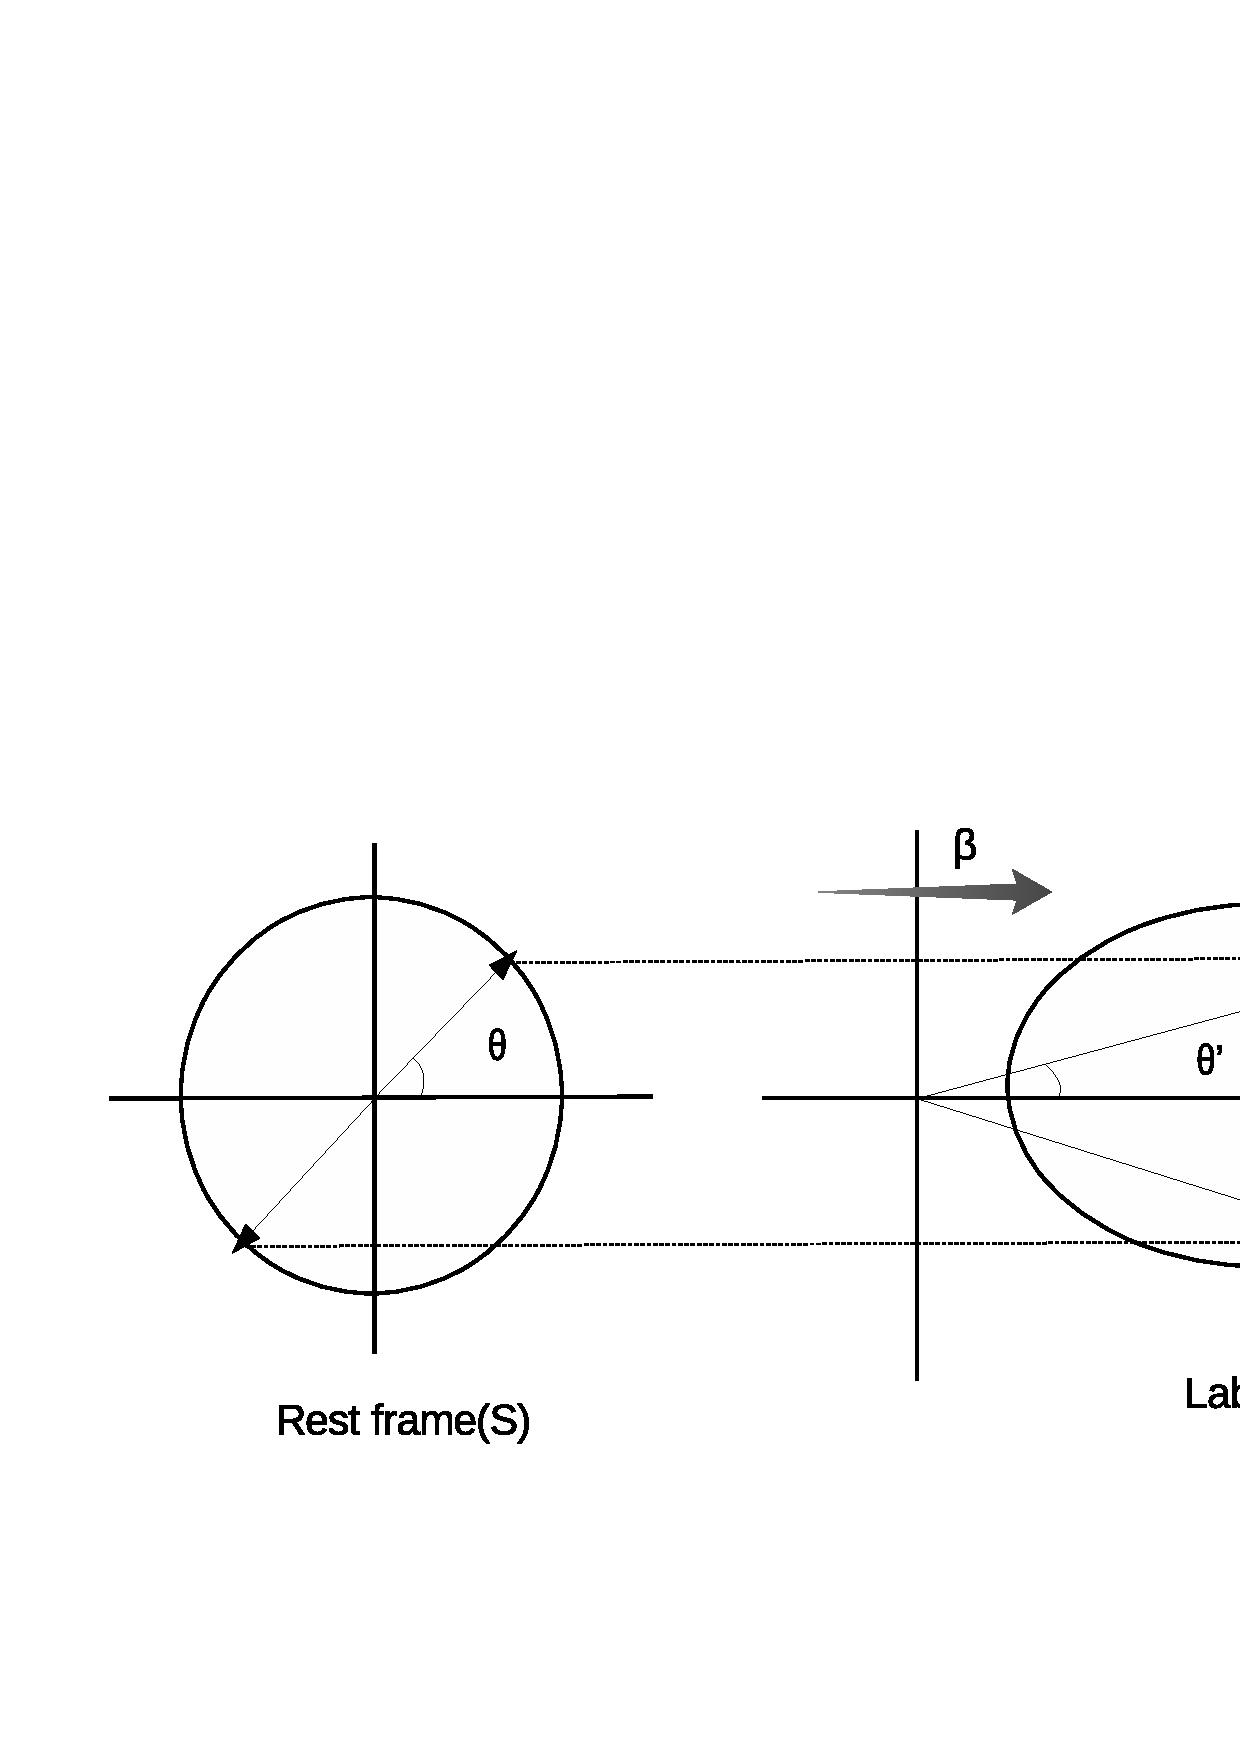
\includegraphics[width=12cm, height=8cm]{3.png}
    \caption{Transformation from $S$ frame to $S^{\prime}$ frame}
    \label{fig:my_label}
\end{figure}
%%%%%%%%%%%%%%%%%%%%%%%%%%%%%%%%%%%%%%%%%%%%%%%%%%%%%%%%%%%%%%%%%%%%%%%%%
\subsection{Invariant Mass}
Invariant mass is useful to find mass of short-live unstable particles from momenta of their observed decay product(e.g $Z\longrightarrow \mu^{+}\mu^{-} \ \ or \ \ e^{+}e^{-} $).

\begin{itemize}
\item 
The invariant mass of a system consisting of $N$ particles is defined as the norm of its total momentum four-vector 
\begin{equation}
    m = \left|\sum_{i=1}^N p_{i}\right|
\end{equation}
\item
Consider $X\longrightarrow a+b$ process, by momentum conservation one can write 
$p_{x} = p_{a}+ p_{b}$, which gives the relation 
\begin{equation}
\begin{split}
        m^2_X c^{2} =& \ \ (p_{a}+p_{b})^2\\
        =&\ \  p_{a}^2 + p_{b}^2 + 2p_{a}.p_{b}\\
        =&\ \  m_{a}^2c^2 + m_{b}^2c^2 + 2E_{a}E_{b}/c^2 -2\Vec{p}_{a}.\Vec{p}_{b}
\end{split}
\end{equation}
\end{itemize}

\section{FCCee: $e^{+}+e^{-}\rightarrow Z+H$ process }
\subsection{Event generator - PYTHIA8}

\begin{itemize}
\item To use Pythia8 we need a Gaudi steering file and a configuration file integrated in $Key4hep$ software stack. The steering file is a python script that is used to configure the Gaudi framework which runs Pythia8. The configuration file is a text file that is used to configure the Pythia8 generator. 
  
% \item We have selected Higgs-strahlung process $(e^{+} + e^{-} \longrightarrow Z + H)$ in production of Higgs by colliding $e^{+}$ and $e^{-}$ beams at center of mass energy $240$GeV.
\item In our case, data has been generated  by selecting Higgs production  $(HiggsSM:ffbar2HZ = on)$ in collision of  $e^{+}(Beams:idA = -11)$ and $e^{-}(Beams:idB = 11)$ collision at center of mass energy  $240$GeV. in pythia command file.



\begin{figure}[ht]
    \centering
    \includegraphics[scale= 0.9]{higgsprocess.png}
    \caption{Higgs-strahlung process}
    \label{fig:hsp}
\end{figure}



\item In  this cases 100000 will be generated and saved in 
ROOT files in $EDM4hep$ format. In order to get there we need 
first to generate the events in $HepMC$ format.

\item In order to get the events in $EDM4hep$ format, we will 
use Gaudi and the tools available in $k4FWCore$ and $k4Gen$. We 
need a Gaudi steering file that reads the $HepMC$ file and writes  out the $EDM4hep$ file format for later processing in $DDSim$.
\end{itemize}


\subsection{FCCee : Full simulation of CLD by DDSim}

\begin{itemize}
  \item We have set up the FCCSW software stack and used $DDSim$ to simulate the detector response of CLD by $/cvmfs/sw-nightlies.hsf.org/key4hep/setup.sh$.
  
  \item  The detectors in FCCSW are described in $DD4hep$ compact files. The compact files are written in XML and expose configuration options for the detector.
  
  \item Then run the simulation with detetor configuration file, event file and steering file and then run reconstruction. 
\end{itemize}

\subsection{Job submission in HTCondor batch system}
The CERN Batch Service is a fairly standard High Throughput Computing (HTC) Batch System with a fair-sharing mechanism.
Its purpose is to allow users to queue up jobs in the system, and maximise the utilisation of the batch farm.
\begin{figure}[h]
  \centering
  \includegraphics[width = 12cm, height = 4cm]{fcc_det/ex1.png}
  \caption{HTCondor}
  \label{fig:my_cond}
\end{figure}

Here we have submit our job to the batch system.The job is 
discrete and independent of other jobs. The job is submitted to 
the batch system and the batch system will run the job and 
return the output to the user. The batch system will also keep 
track of the jobs and their status.
\begin{itemize}
  \item HTCondor provides the ability to match executables files using regular expressions and add a job to the queue for each file. 
  \item In our case we have queued 10 jobs for respective $.sh$ executable file.The 10 jobs, even if they have different executables, have the same Cluster and different ProcIds.
\end{itemize}


\subsection{Analysis of Delphes samples$^{\cite{fcc}}$}
We have used Delphes sample  to get the detector response of CLD. Delphes is a fast detector 
simulation framework. It is based on the fast simulation package FastJet and uses the ROOT data 
analysis framework.
The FCCAnalyses framework is based on the RDataFrame interface which allows fast and efficient 
analysis of ROOT's TTrees and on samples following the $EDM4HEP$ event data model.
Here we have produced   flat ntuples with observables of interest and then 
produced plots with FCCAnalyses.

\chapter{\label{result}Result and Disscusion}

\setcounter{equation}{0}
\setcounter{table}{0}
\setcounter{figure}{0}
% \baselineskip 16pt
\hspace{10pt}\\

\section{$Z\longrightarrow \mu^{+} + \mu^{-}$ process}
\begin{figure}[ht!]
    \centering
    \includegraphics[width=0.5\linewidth]{plots/plots/mue.png}\hfill
    \includegraphics[width=0.5\linewidth]{plots/plots/mup.png}
    \caption{Energy and momentum distribution of $\mu^{+}$ and $\mu^{-}$ at 240GeV.}
\end{figure}

\begin{figure}[ht!]
    \centering
    \includegraphics[width=0.5\linewidth]{plots/plots/mupt.png}\hfill
    \includegraphics[width=0.5\linewidth]{plots/plots/muy.png}
    \caption{Transverse momentum and rapidity  distribution of $\mu^{+}$ and $\mu^{-}$ at 240GeV.}
\end{figure}

\begin{figure}[ht!]
    \centering
    \includegraphics[width=0.5\linewidth]{plots/plots/zmu_m.png}\hfill
    \includegraphics[width=0.5\linewidth]{plots/plots/zmu_charge.png}
    \caption{Reconstructed mass and charge  from  $\mu^{+}$ and $\mu^{-}$ at 240GeV.}
    \label{fig:zmu_mass}
\end{figure}

\begin{figure}[ht!]
    \centering
    \includegraphics[width=0.5\linewidth]{plots/plots/zmu_theta.png}\hfill
    \includegraphics[width=0.5\linewidth]{plots/plots/zmu_y.png}
    \caption{Reconstructed $\theta$ and rapidity  from  $\mu^{+}$ and $\mu^{-}$ at 240GeV.}
\end{figure}

\begin{figure}[ht!]
    \centering
    \includegraphics[width=0.5\linewidth]{plots/plots/zmu_pt.png}\hfill
    \includegraphics[width=0.5\linewidth]{plots/plots/zmu_recoil_m.png}
    \caption{Reconstructed transverse momentum and recoil mass  from  $\mu^{+}$ and $\mu^{-}$ at 240GeV.}
\end{figure}



\section{$Z\longrightarrow e^{+} + e^{-}$ process}



\begin{figure}[ht!]
    \centering
    \includegraphics[width=0.5\linewidth]{plots/plots/ee.png}\hfill
    \includegraphics[width=0.5\linewidth]{plots/plots/ep.png}
    \caption{Energy and momentum distribution of $e^{+}$ and $e^{-}$ at 240GeV.}   
\end{figure}

\begin{figure}[ht!]
    \centering
    \includegraphics[width=0.5\linewidth]{plots/plots/ept.png}\hfill
    \includegraphics[width=0.5\linewidth]{plots/plots/ey.png}
    \caption{Transverse momentum and rapidity distribution of $e^{+}$ and $e^{-}$ at 240GeV.}                      
\end{figure}


\begin{figure}[ht!]
    \centering
    \includegraphics[width=0.5\linewidth]{plots/plots/z_e_m.png}\hfill
    \includegraphics[width=0.5\linewidth]{plots/plots/z_e_charge.png}
    \caption{Reconstructed mass and charge  from  $e^{+}$ and $e^{-}$ at 240GeV.}
    \label{fig:z_e_m}
\end{figure}    
\clearpage

\begin{figure}[ht!]
    \centering
    \includegraphics[width=0.5\linewidth]{plots/plots/z_e_theta.png}\hfill
    \includegraphics[width=0.5\linewidth]{plots/plots/z_e_y.png}
    \caption{Reconstructed $\theta$ and rapidity  from  $e^{+}$ and $e^{-}$ at 240GeV.}
\end{figure}    

\begin{figure}[ht!]
    \centering
    \includegraphics[width=0.5\linewidth]{plots/plots/z_e_pt.png}\hfill
    \includegraphics[width=0.5\linewidth]{plots/plots/z_e_recoil_m.png}
    \caption{Reconstructed transverse momentum and recoil mass  from  $e^{+}$ and $e^{-}$ at 240GeV.}
\end{figure}

From figure(\ref{fig:zmu_mass}) and (\ref{fig:z_e_m}) we have got the distributions of the reconstructed Z  mass for $Z\longrightarrow \mu^{+} + \mu^{-}$ and $Z\longrightarrow e^{+} + e^{-}$ respectively.  A peak can be seen around 91GeV. in both distributions, which matches the Z boson mass.

%\section{$H \longrightarrow b + \Bar{b}$ process}
%\section{$e^{+} + e^{-} \longrightarrow H + Z$ process}

%%%%%%%%%%%%%%%%%%%%%%%%%%%%%%%%%%%%%%%%%%%%%%%%%%%%%%%%%%%%%%%%%%%%%%%%%%%%%%
\chapter{\label{summary}Conclusion}

\setcounter{equation}{0}
\setcounter{table}{0}
\setcounter{figure}{0}
\baselineskip 24pt
\hspace{10pt}
\\

We  have reconstructed  the mass of $Z$ boson from  $e^{+}e^{-}$, $\mu^{+}\mu^{-}$   in decay of $Z$ which satisfies invariant mass law  and also studied different kinematic parameter as shown in previous section.
The analysis performed by  running  a fast parametric detector simulation with Delphes in the EDM4Hep format. Then 
we have 
applied  an event selection on our delphes sample with FCCAnalyses
and  produced flat ntuples with observables of interest with FCCAnalyses.
By analysing the  ntuple  produced with ROOT's RDataFrame
and  used  the  ROOT's  TTree  class  to  store  the  data  in  a  tree  structure  and  then  used  the  ROOT's  TCanvas  class  to  plot  the  data  in  a  graph  format.
\chapter{Future study}

\setcounter{equation}{0}
\setcounter{table}{0}
\setcounter{figure}{0}
\baselineskip 24pt
\hspace{10pt}
\\

We will generate the signal with background samples and apply fast parametric detector simulation with Delphes in the EDM4Hep format, then  analysis it as we have done in this project. We will also study the different kinematics of Higgs boson and its daughter particles. Later we will study the tracking efficiency  and jet energy resolution of the detector.
\newcommand{\bib}{\bibitem}
%\newcommand{\bibitem}

\clearpage
\addcontentsline{toc}{chapter}{References}
% \baselineskip 24pt
% \hspace{10pt}
% \\
\begin{thebibliography}{9}

\bibitem{CLD}The CLD Detector Concept-
\url{https://indico.cern.ch/event/1064327/contributions/4893180/attachments/2452299/4204992/220601_FCCWeek_CLD_sailer.pdf}

\bibitem{fcc}
\url{https://github.com/HEP-FCC/FCCeePhysicsPerformance/blob/master/General/README.md#How-to-associate-RecoParticles-with-Monte-Carlo-Particles}

\bibitem{}
\url{https://hep-fcc.github.io/fcc-tutorials/fast-sim-and-analysis/FccFastSimGeneration.html}


\bibitem{} Bacchetta, N., et al. "CLD -- A Detector Concept for the FCC-ee." arXiv, 2019, \url{https://doi.org/10.48550/arXiv.1911.12230}. Accessed 25 Nov. 2022.



\end{thebibliography}

%\baselineskip 15pt
%\setlength{\parskip}{10pt}



%%\clearpage
%\addcontentsline{toc}{chapter}{Appendices}
\begin{appendices}
\chapter{\label{appendix}The Code for generating data from
PYTHIA for $e^{+}+e^{-}\rightarrow Z + H$}
\end{appendices}

\setcounter{equation}{0}
\setcounter{table}{0}
\setcounter{figure}{0}
\baselineskip 10pt
\lstinputlisting[language = C++]{HiggsSt.cc}



%}
\end{document}
